\documentclass[11pt]{article}

\newcommand{\wshop}{
    1
}
\newcommand{\subtitle}{
    Automata and Languages
}

% Page Setup
\usepackage{geometry}
\geometry{
    a4paper,
    margin={2.5cm}
}

% Basic Packages
\usepackage{amssymb}
\usepackage{stmaryrd}
\usepackage{amsmath}
\usepackage{amsthm}
\usepackage{mathtools}
\usepackage{mathpartir}
\usepackage{enumitem}
\usepackage{mathabx}

% Font
\usepackage{charter}

% Bibliography and index
\usepackage[backend=biber, style=numeric]{biblatex}
\addbibresource{refs.bib}
\usepackage{makeidx}
\makeindex

% Colors and Graphics
\usepackage[dvipsnames, x11names]{xcolor}
\usepackage{tikz}
\usetikzlibrary{
    cd,
    fit,
    calc,
    positioning,
    arrows,
    automata,
    shapes
}
\tikzset{
    baseline = (current bounding box.center),
    every state/.append style = {
        rectangle,
        rounded corners=5pt,
		inner sep = 3pt,
		minimum size = 18pt,
		initial text = {},
        fill=Azure1
	},
	every edge/.append style = {
		->,
		>=stealth,
		bend angle=10,
		thick
	}
}
\usepackage{musicography}
\usepackage{graphicx}
\usepackage{svg}
\graphicspath{../imgs/}

% Hyperlinks
\usepackage{hyperref}
\hypersetup{
    colorlinks,
    linkcolor   = black,
    filecolor   = RubineRed,
    urlcolor    = RubineRed,
    citecolor   = RubineRed,
    pdftitle    = {Notes on Behavioural PDEs}
}
\usepackage[capitalize]{cleveref}

% Environments
\theoremstyle{theorem} % In Italics
\newtheorem{theorem}                    {{\color{Purple}Theorem}}[section]
\newtheorem{lemma}          [theorem]   {{\color{Magenta}Lemma}}
\newtheorem{proposition}    [theorem]   {Proposition}
\newtheorem{corollary}      [theorem]   {Corollary}
\newtheorem{question}                   {{\color{red}Question}}

\theoremstyle{definition} % Not in italics
\newtheorem{definition}     [theorem]   {{\color{NavyBlue}Definition}}
\newtheorem{example}        [theorem]   {{\color{ForestGreen}Example}}
\newtheorem{problem}                    {{\color{BurntOrange}Problem}}

\theoremstyle{remark} % Subdued label
\newtheorem{remark}[theorem]        {{\color{Gray}Remark}}

% (1), (2), ...
\renewcommand\labelenumi{(\theenumi)}

% Go nuts with line breaks 
\allowdisplaybreaks

%%%%%%%%%%
% MACROS %
%%%%%%%%%%

\newcommand{\op}{\mathrm{op}}               % Opposite
\newcommand{\inv}{{-1}}                     % Inverse
\newcommand{\id}{\mathsf{id}}               % Identity f(x) = x
\newcommand{\Det}{\mathrm{Det}}             % determinize
\newcommand{\Lang}{\mathcal{L}}             % Language

\newcommand{\incl}{\mathsf{incl}}           % Inclusion
\newcommand{\proj}{\mathsf{proj}}           % Projection

% Numbers and Standard notation
\newcommand{\NN}{\mathbb{N}}                % 0, 1, 2, 3, 4, ...
\newcommand{\ZZ}{\mathbb{Z}}                % ..., -2, -1, 0, 1, 2, ...
\newcommand{\QQ}{\mathbb{Q}}                % n/m for n and m in \NN and m > 0
\newcommand{\RR}{\mathbb{R}}                % real numbers
\newcommand{\pRR}{\mathbb{R}_{+}}           % positive real numbers

\newcommand{\dom}{\mathrm{dom}}             % Domain
\newcommand{\cod}{\mathrm{cod}}             % Codomain

\newcommand{\Grph}{\operatorname{Grph}}     % Graph of a function

% Transitions
\newcommand{\tr}[1]{
    \mathrel{
        \raisebox{-1pt}{
            \(\xrightarrow{#1}\)
        }
    }
}
\newcommand{\bisim}{\mathrel{\raisebox{1pt}{\(\underline{\leftrightarrow}\)}}}

% Text
\newcommand{\code}[1]{\texttt{#1}}
\newcommand{\codeblock}[1]{
    \begin{center}
        \parbox{0.8\textwidth}{
            \ttfamily
            #1
        }
    \end{center}
}

% Boolean statements
\newcommand{\OR}{~\mathrm{or}~}
\newcommand{\AND}{~\mathrm{and}~}
\newcommand{\NOT}{\mathrm{not}~}
\newcommand{\IMPLIES}{~\mathrm{implies}~}
\newcommand{\FORALL}{\mathrm{for\ all}~}
\newcommand{\EXISTS}{\mathrm{there\ exists}~}
\newcommand{\SUCHTHAT}{~\mathrm{such\ that}~}



% Title
\title{CSCI 341 Workshop \wshop}
\author{\subtitle}
\date{
    \today
}

\pagestyle{empty}

\begin{document}


\maketitle

%%%%%%%%%%%%%%%%%%%%%%%%%%%%%%%%%%%%%%%%%%%%%%%%%%%%%%%%%%%%
% START OF WORK SHOP.                                      %
%%%%%%%%%%%%%%%%%%%%%%%%%%%%%%%%%%%%%%%%%%%%%%%%%%%%%%%%%%%%

\begin{theorem}
    [Ordinary Induction]
    Let \(S \subseteq \mathbb{N}\) be a set of natural numbers.
    If the following two statements are true:
    \begin{description}
        \item[Base Case] The number \(0 \in S\).
        \item[Induction Step] If the number \(n \in S\), then the number \(n + 1 \in S\).
    \end{description}
    then \(S = \mathbb{N}\).
\end{theorem}

\begin{problem}
    [Counting Trees]
    Recall that a complete binary tree is a binary tree in which every level of the tree is entirely full. 
    For example, the following tree is a complete binary tree with three levels.
    \[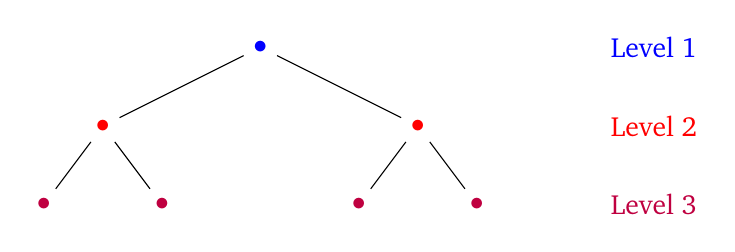
\begin{tikzpicture}
        \node[blue] (level1) at (5, 0) {Level 1};
        \node[blue] (root) at (0,0) {\(\bullet\)};

        \node[red] (level1) at (5, -1) {Level 2};
        \node[red] (0) at (-2,-1) {\(\bullet\)};
        \node[red] (1) at (2,-1) {\(\bullet\)};

        \node[purple] (level1) at (5, -2) {Level 3};
        \node[purple] (00) at (-2.75,-2) {\(\bullet\)};
        \node[purple] (01) at (-1.25,-2) {\(\bullet\)};
        \node[purple] (10) at (1.25,-2) {\(\bullet\)};
        \node[purple] (11) at (2.75,-2) {\(\bullet\)};

        \draw (root) 
            -- (0) 
            -- (00) 
            -- (0) 
            -- (01) 
            -- (0) 
            -- (root) 
            -- (1)
            -- (10)
            -- (1)
            -- (11);
    \end{tikzpicture}\]
    The complete tree with three layers has \(7\) nodes. 
    Using \emph{Ordinary Induction}, prove that the complete binary tree with \(n\) layers has \(2^n - 1\) nodes.
    For example, \(2^3 - 1 = 8 - 1 = 7\).
\end{problem}

\begin{problem}
    [*Bonus* Counting Prefixes]
    Given a word \(w = a_0a_1\cdots a_{n-1}\), a \emph{subword} of \(w\) is a consecutive sequence of indices \([k, k+1, k+ 2, \dots, l - 1]\) for \(0 \le k \le n-1\).
    We often identify a subword with the word \(u = a_{k}a_{k+1}\cdots a_{l-1}\), so that there exist two other subwords \(v_1\) and \(v_2\) such that \(w = v_1uv_2\).
    \[
        \underbrace{a_0 a_1 a_2 \cdots a_{n-1}}_{w}
        = \underbrace{a_0 a_1 \cdots a_{k-1}}_{v_1}
        \underbrace{a_{k} a_{k+1} \cdots a_{l-1}}_{u}
        \underbrace{a_{l} a_{l+1} \cdots a_{n-1}}_{v_2}
    \]
    For example, the subwords of \(aba\) are \[
        \underbrace{[]}_\varepsilon, 
        \underbrace{[0]}_{a},
        \underbrace{[1]}_{b},
        \underbrace{[2]}_{a},
        \underbrace{[0, 1]}_{ab},
        \underbrace{[1, 2]}_{ba},
        \underbrace{[0, 1, 2]}_{aba}
    \]
    of which there are \(7\).
    Using Ordinary Induction, prove that a word of length \(n\) has
    \[
        \frac{n(n+1) + 2}{2}
    \] 
    many subwords.
    \emph{Hint: Every subword of the word \(wa\) is either a subword of \(w\) or a suffix of \(wa\), i.e., ends with \(a\).
    also, \((n+1)(n+2) = n^2 + 3n + 2\)}.
\end{problem}

\pagebreak

\noindent\emph{Solution to Counting Trees.}
    Let \[
        S = \{n \mid \text{the complete binary tree with \(n\) layers has \(2^n - 1\) nodes}\}
    \]
    Our goal is to prove that \(S = \NN\).
    We proceed by induction on \(n\).
    \bigskip

    \noindent\textbf{Base Case}
    
    \vspace*{5em}

    \noindent\textbf{Induction Hypothesis}

    \vspace*{10em}

    \noindent\textbf{Induction Step:}
    
\vfill\hfill\(\Box\)
\pagebreak

\noindent\emph{Solution to Counting Subwords.}
    We proceed by induction on \(n\).
    \bigskip

    \noindent\textbf{Base Case}
    
    \vspace*{5em}

    \noindent\textbf{Induction Hypothesis}

    \vspace*{10em}

    \noindent\textbf{Induction Step:}
    
\vfill\hfill\(\Box\)
\pagebreak

\begin{theorem}
    [Induction on Words]
    Let \(L \subseteq A^*\) be a language. 
    If the following two statements are true:
    \begin{description}
        \item[Base Case] The empty word \(\varepsilon \in L\) is in the language.  
        \item[Induction Step] If \(w \in L\), then for any \(a \in A\), \(wa \in L\).  
    \end{description}
    then \(L = A^*\).
\end{theorem}

\begin{problem}
    [Double-reversal]
    Given a word \(w\), define \(w^\op\) to be the \emph{reversal} of the word, as follows:
    on the empty word, we define \(\varepsilon^\op = \varepsilon\). 
    Given a word \(w \in A^*\) and a letter \(a \in A\), we define \((wa)^\op = a w^\op\).
    % \((a_0 a_1 \cdots a_{n-1})^\op = a_{n-1}\cdots a_1 a_0\).
    % Note that \(\varepsilon^\op = \varepsilon\) by definition.
    Use Induction on Words to prove that for any word \(w \in A^*\), \((w^\op)^\op = w\). 
\end{problem}

\begin{problem}
    [All-accepting]
    Let \(A = \{0,1\}\).
    Use Induction on Words to prove that the all-accepting automaton accepts every word form \(A\). 
    That is, 
    \[
    \mathcal A_{\checkmark} = 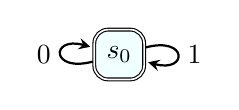
\begin{tikzpicture}
        \node[state, accepting] (0) at (0, 0) {\(s_0\)};
        \draw[loop] (0) edge[loop right] node[right] {\(1\)} (0);
        \draw[loop] (0) edge[loop left] node[left] {\(0\)} (0);
    \end{tikzpicture}
    \qquad 
    \Lang(\mathcal A_\checkmark, s_0) = A^*
    \]
\end{problem}

\begin{problem}
    [*Bonus* Double Double Reversal]
    Use Induction on Words to prove that for all \(w,u \in A^*\), the reversal of their concatenation is the reversed concatenation of their reversals: \[(wu)^\op = u^\op w^\op\]
\end{problem}

\pagebreak

\noindent\emph{Solution to Double Reversal.}
    Let \(L = \{w \mid (w^\op)^\op = w\}\).
    The goal is to show that \(L = A^*\).
    We proceed by induction on \(w \in L\).
    \bigskip

    \noindent\textbf{Base Case}
    
    \vspace*{5em}

    \noindent\textbf{Induction Hypothesis}

    \vspace*{10em}

    \noindent\textbf{Induction Step:}
    
\vfill\hfill\(\Box\)


\pagebreak

\noindent\emph{Solution to All-accepting.}
    Let \(L = \Lang(\mathcal A_{\checkmark}, s_0)\).
    The goal is to show that \(L = A^*\).
    We proceed by induction on \(w \in L\).
    \bigskip

    \noindent\textbf{Base Case}
    
    \vspace*{5em}

    \noindent\textbf{Induction Hypothesis}

    \vspace*{10em}

    \noindent\textbf{Induction Step:}
    
\vfill\hfill\(\Box\)

\pagebreak

\noindent\emph{Solution to Double Double Reversal.}
    This one is a bit trickier than Double Reversal, because there are two words involved in the statement. 
    Interestingly, we only need to involve one of the words in the proof:
    Let \[
        L = \{w \mid \text{for any word \(u\), \((wu)^\op = u^\op w^\op\)}\}
    \]
    The goal is to show that \(L = A^*\).
    We proceed by induction on \(w \in L\).
    \bigskip

    \noindent\textbf{Base Case}
    
    \vspace*{5em}

    \noindent\textbf{Induction Hypothesis}

    \vspace*{10em}

    \noindent\textbf{Induction Step:}
    
\vfill\hfill\(\Box\)


\end{document}